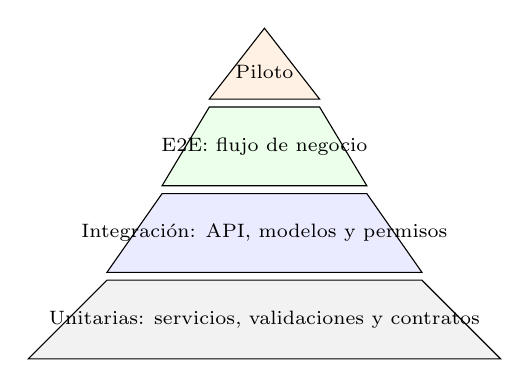
\begin{tikzpicture}[every node/.style={font=\scriptsize}]
\draw[fill=gray!10] (0,0) -- (6,0) -- (5,1) -- (1,1) -- cycle; \node at (3,0.5) {Unitarias: servicios, validaciones y contratos};
\draw[fill=blue!8] (1,1.1) -- (5,1.1) -- (4.3,2.1) -- (1.7,2.1) -- cycle; \node at (3,1.6) {Integración: API, modelos y permisos};
\draw[fill=green!8] (1.7,2.2) -- (4.3,2.2) -- (3.7,3.2) -- (2.3,3.2) -- cycle; \node at (3,2.7) {E2E: flujo de negocio};
\draw[fill=orange!10] (2.3,3.3) -- (3.7,3.3) -- (3,4.2) -- cycle; \node at (3,3.65) {Piloto};
\end{tikzpicture}
